% Week 9 report: naive result and failure argument (P5, positive-unlabelled wiring).
% Numbers come from numbers.tex, written by scripts/week9_report_numbers.py; figures from figures/week9/.
\documentclass[conference]{IEEEtran}
\usepackage{amsmath,amssymb,graphicx,booktabs,url}
\newcommand{\CPrimary}{0.656}
\newcommand{\BrierNaive}{3.866}
\newcommand{\MeanPNaive}{0.0027}
\newcommand{\BrierNaiveC}{3.899}
\newcommand{\MeanPNaiveC}{0.0041}
\newcommand{\BrierPU}{3.910}
\newcommand{\MeanPPU}{0.0041}
\newcommand{\BrierBase}{3.983}
\newcommand{\MeanPBase}{0.0026}
\newcommand{\MeanY}{0.0040}
\newcommand{\PairsBelowFive}{at least 90\%}
\newcommand{\TestDzero}{106/238 groups positive, $p=0.105$, mean $-0.100$ $[-0.256, 0.010]\times10^{-3}$}
\newcommand{\TestDone}{109/238 groups positive, $p=0.218$, mean $-0.088$ $[-0.235, 0.016]\times10^{-3}$}
\newcommand{\TestDtwo}{137/238 groups positive, $p=0.046$, mean $0.011$ $[-0.005, 0.032]\times10^{-3}$}
\newcommand{\PooledDzero}{$-0.032$}
\newcommand{\PooledDone}{$-0.044$}
\newcommand{\PooledDtwo}{$-0.011$}
\newcommand{\TopPQone}{0.026}
\newcommand{\TopYQone}{0.030}
\newcommand{\LevelNaive}{0.67}
\newcommand{\TopPNaive}{0.017}
\newcommand{\LevelNaiveC}{1.02}
\newcommand{\TopPNaiveC}{0.026}
\newcommand{\LevelPU}{1.02}
\newcommand{\TopPPU}{0.026}
\newcommand{\TopY}{0.030}
\newcommand{\LevelNaiveSD}{0.11}
\newcommand{\AUCNaive}{0.923}
\newcommand{\AUCPU}{0.924}
\newcommand{\RunTimes}{mean over 25 runs on 8 CPU cores, no thinning ($q=1$) 18~min; synapse $q=0.7$ (primary) 33~min}
\newcommand{\LevelQone}{1.02}
\newcommand{\BrierQone}{3.869}
\newcommand{\AUCQone}{0.928}
\newcommand{\Recorded}{32{,}125}
\newcommand{\MissedMid}{20{,}100}
\newcommand{\MissedLo}{30{,}300}
\newcommand{\MissedHi}{9{,}700}
\newcommand{\EdgesSentence}{on 171 shared cell types, 9.2 outgoing partners per neuron in FAFB and 19.7 in MaleCNS at $\tau=10$ (ratio 2.13), 9.8 at $\tau=18$ (ratio 1.06)}

\newcommand{\E}{\mathbb{E}}

\begin{document}
\title{Recorded Is Not Connected: a Naive Link Predictor on the Fly Central Complex and Why Its Probabilities Are Off by $c$}
\author{\IEEEauthorblockN{Tarkan Eyerci}\IEEEauthorblockA{CENG8004 Machine Learning, Project 5 (Week 9 milestone)\\
Code: \url{\RepoURL} (tag \texttt{week9})}}
\maketitle

\begin{abstract}
A connectome records a connection only where enough synapses were detected, so ``not recorded'' mixes absent and missed connections. We fit the standard tool, a weighted logistic regression with unrecorded pairs as negatives, on the FAFB central complex (2{,}875 neurons, $\tau=10$ synapses), together with its rescaled version $\min(g/c,1)$ and a positive-unlabelled (PU) fit, on a dropout benchmark where the true labels are known. We derive that the naive model estimates $c\,P(y{=}1\mid x)$ rather than $P(y{=}1\mid x)$: its ranking is nearly right and its level is wrong by the label frequency $c$. On the benchmark \HeadlineSentence
\end{abstract}

\section{The naive result}
\subsection{Question and locked set-up}
The question is the probability that a neuron pair is truly connected ($y=1$: at least $\tau$ synapses in the true graph) given its features $x$, when only recorded connections ($s=1$) are observed. All choices follow the revised lock note (page 1 and addendum A1--A8); we cite them by item. Population: the FAFB central-complex roster (2{,}875 neurons, 238 homologue groups), $\tau=10$, labels from region-pair synapse counts (page 1). Features: identity, cell type, region, degree and spatial groups, built from the training graph only, held-out numerics clipped to the training range (page 1, A6). Sampling: every recorded pair and about 20 unlabelled pairs per positive, with Horvitz--Thompson weights. Split: five folds of homologue groups, so both members of a mirror type are held out together; seeds 10--14, each with its own folds, thinning and sample (A2). MaleCNS is not fitted (A7, page 1): the model runs on FAFB only, and edges per neuron in the two datasets are compared descriptively (\EdgesSentence).

\textbf{Benchmark.} The truth $y$ is the recorded FAFB graph; we thin it and score against the full graph. Primary condition: synapse dropout with keep probability $q=0.7$ (each synapse kept independently; a connection survives if $\ge\tau$ synapses remain). Secondary: connection dropout $q=0.7$, synapse dropout $q=0.5$, and $q=1$ (no thinning; the real-data run). The realised label frequency $c$ is the share of true positives among training sources still recorded (A2).

\textbf{Models} (A1). Baseline: intercept only (the weighted recorded rate). Naive: scikit-learn 1.7.2 \texttt{LogisticRegression} (lbfgs, L2, $C=1/(\lambda\sum_i a_i)$, sample weights $a_i$). Naive/$c$: $\min(g/c,1)$ \cite{elkan2008}. PU: the same logistic model fitted with target $s/c$ (A8, a stated deviation: week 9 also forbids from-scratch numbers). Each model's $\lambda\in\{10^{-2},\dots,10^{-7}\}$ comes from 3-fold inner cross-validation over homologue groups on the training sources only, scored on $s$ (log-loss of $g$, of $\min(g,c)$, and of $c\,f_{\rm PU}$), with the one-standard-error rule. No choice uses the test folds; tuning losses use only $s$, and the training sources' true labels enter only as the benchmark's known $c$ (A2).

\subsection{Results}
Table~\ref{tab:main} gives the 25 runs (5 seeds $\times$ 5 folds) per condition as mean and SD. \ResultsParagraph

\begin{table}[t]\centering\caption{Held-out scores against the true labels $y$, mean (SD) over 25 runs. Brier $\times10^{3}$. Naive and naive/$c$ rank alike where they share $\lambda$, up to ties from the clip at 1; each is computed separately.}\label{tab:main}
\begin{tabular}{@{}llrrrr@{}}\toprule
condition & model & Brier & mean $p$ & AUC & AP\\\midrule
no thinning ($q=1$) & baseline & 3.980 (0.952) & 0.0039 (0.0002) & 0.5 & --\\
 & naive & 3.869 (0.921) & 0.0041 (0.0008) & 0.928 (0.019) & 0.078 (0.031)\\
 & naive/$c$ & 3.869 (0.921) & 0.0041 (0.0008) & 0.928 (0.019) & 0.078 (0.031)\\
 & PU & 3.869 (0.921) & 0.0041 (0.0008) & 0.928 (0.019) & 0.078 (0.031)\\
\midrule
synapse $q=0.7$ (primary) & baseline & 3.983 (0.956) & 0.0026 (0.0002) & 0.5 & --\\
 & naive & 3.866 (0.918) & 0.0027 (0.0006) & 0.923 (0.020) & 0.076 (0.029)\\
 & naive/$c$ & 3.899 (0.954) & 0.0041 (0.0009) & 0.923 (0.020) & 0.076 (0.029)\\
 & PU & 3.910 (0.963) & 0.0041 (0.0010) & 0.924 (0.019) & 0.075 (0.028)\\
\bottomrule
\end{tabular}

\end{table}

\begin{figure}[t]\centering
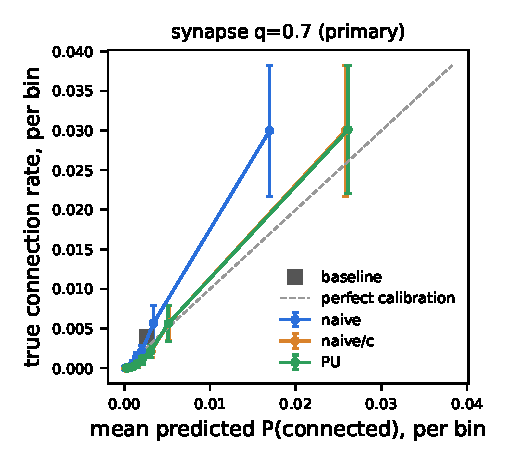
\includegraphics[width=\columnwidth]{../../figures/week9/fig1_reliability_synapse_q0.7.pdf}
\caption{\FigOneCaption}\label{fig:rel}
\end{figure}

\section{The failure argument}
\subsection{The target}
For a pair with features $x$ let $y\in\{0,1\}$ be the true connection and $s\in\{0,1\}$ the recorded one; $s=1$ implies $y=1$. The question needs
\begin{equation}
f(x)=P(y=1\mid x),
\end{equation}
a calibrated connection probability, and we judge an estimate $p$ by the Brier score against $y$, $B(p)=\sum_i a_i (p_i-y_i)^2/\sum_i a_i$, a proper score: in expectation it cannot prefer a model for under-predicting. Under \emph{selected completely at random} (SCAR) labelling a true connection is recorded with a constant probability $c$, independent of $x$: $P(s=1\mid y=1,x)=c$. Then
\begin{equation}
g(x)\equiv P(s=1\mid x)=c\,f(x).\label{eq:scar}
\end{equation}

\subsection{What the naive method computes}
With sample weights $a_i$, scikit-learn's \texttt{LogisticRegression} with the default L2 penalty minimises \cite{sklearn}
\begin{equation}
C\sum_i a_i\,\ell(s_i,\sigma(z_i))+\tfrac12\lVert w\rVert^2,\quad z_i=w^\top x_i+b,
\end{equation}
with $\ell(s,p)=-s\ln p-(1-s)\ln(1-p)$ and the intercept $b$ unpenalised for lbfgs (liblinear would penalise it). Dividing by $C\sum_i a_i$ and setting $\lambda=1/(C\sum_i a_i)$ gives the weighted mean log-loss plus $(\lambda/2)\lVert w\rVert^2$. Its label is $s$, not $y$, and because of the penalty its coefficients cannot be compared one by one with those of an unpenalised fit. As $\lambda\to0$ and with a correctly specified model, the minimiser of the expected log-loss is $\sigma(z(x))=g(x)$ (Appendix~A). So the naive model estimates $g=c f$, not $f$.

\subsection{The gap}
\textbf{Level.} At the optimum the derivative with respect to the unpenalised $b$ is zero:
\begin{equation}
\sum_i a_i\big(\sigma(z_i)-s_i\big)=0\ \Rightarrow\ \frac{\sum_i a_i\sigma(z_i)}{\sum_i a_i}=\frac{\sum_i a_i s_i}{\sum_i a_i},\label{eq:level}
\end{equation}
the mean fitted probability equals the recorded rate, which is $c$ times the true rate in expectation. A correction with the true $c$ restores the level by construction (up to the clip at 1); the PU fit has the same identity with $s$ replaced by $s/c$, so its weighted mean training prediction is $P(s=1)/c$, and naive/$c$ and PU share a level for the same reason; a level recovered this way shows that $c$ was right, not that the method is.

\textbf{Ranking.} For rare probabilities the factor $c$ is an intercept shift. Writing $\sigma(z)=e^z/(1+e^z)$,
\begin{equation}
\frac{c\,\sigma(z)}{\sigma(z+\ln c)}=\frac{1+c\,e^z}{1+e^z}=1-(1-c)\,\sigma(z),\label{eq:shift}
\end{equation}
so $c\,\sigma(z)=\sigma(z+\ln c)$ up to a relative error $(1-c)\sigma(z)$, below $0.05(1-c)$ wherever $\sigma(z)\le0.05$ (under SCAR the weighted mean of $f$ over the training pairs is $P(s=1)/c$, estimated by the weighted recorded rate; by Markov's inequality $f\le0.05$ for \PairsBelowFive\ of them in every run). A logistic model for $f$ and one for $cf$ then differ almost only in $b$: the naive model ranks pairs nearly as the true model does. Since $\min(g/c,1)$ is non-decreasing in $g$, naive/$c$ built on the same fit keeps the naive order, except that pairs with $g\ge c$ tie at 1; with its own $\lambda$ (A1) it can differ, so we report AUC and AP for each.

\textbf{Brier cost.} For a fixed $x$ and a prediction $p$, $\E[(p-y)^2\mid x]=f(1-f)+(p-f)^2$ (Appendix~B). The population naive prediction $p=cf$ therefore costs an extra $(1-c)^2 f^2$, and on average
\begin{equation}
B(\text{naive})-B(f)=(1-c)^2\,\E[f^2],
\end{equation}
which is tiny when $f$ is small. Rescaling removes this bias but scales the estimation noise: if $\hat g=g+\varepsilon$ with $\E\varepsilon=0$, $\operatorname{Var}\varepsilon=v(x)$, then (ignoring the clip)
\begin{equation}
B(\hat g/c)-B(\hat g)\approx\E\!\left[v\Big(\frac1{c^2}-1\Big)\right]-(1-c)^2\E[f^2],\label{eq:tradeoff}
\end{equation}
so the rescaled model wins only where the squared bias exceeds the extra variance. The comparison can go either way and depends on $\lambda$ through $v$; this is why we show reliability curves beside the Brier score.

\textbf{Non-constant $c$.} If detection depends on strength, $c=c(x)$ and $g=c(x)f(x)$. Dividing by one constant $\bar c$ leaves the bias $f(x)\big(c(x)/\bar c-1\big)$: pairs with weak connections ($c(x)<\bar c$) stay under-predicted and strong ones become over-predicted. Neither naive nor naive/$c$ can remove this term, because it is not in their objective.

\textbf{What a fix optimises.} Replacing the label $s$ by $s/c$ in the log-loss gives, per $x$, the expected loss $-\tfrac{g}{c}z+\ln(1+e^z)$, minimised at $\sigma(z)=g/c=f$ (Appendix~C): the convex PU risk \cite{duplessis2015} targets $f$ directly, but only for the right $c$.

\subsection{When they coincide}
If $c=1$ every connection is recorded, $g=f$, and the naive, naive/$c$ and PU objectives are identical; this case is the verification of the week 11 implementation (a unit test already compares the PU code with scikit-learn at $c=1$). The run at $q=1$ is this case on the benchmark.

\subsection{The evidence}
\EvidenceParagraph

\textbf{$c$ on the real data.} The mirror estimate is $\hat c=0.63$ (95\% interval 0.53--0.71, bootstrap over source cell types) at $\tau=10$: of 267 recorded pairs among the 110 neurons in one-per-side types, 168 have their mirror pair recorded too. Of the 99 unrecorded mirror pairs, 13 have no synapse on the other side and 86 have 1 to 9. Both groups mix causes. A connection that loses synapses to detection (a miss, $y=1$, $s=0$) falls in the second group, which is what synapse dropout models; the first group holds connections lost entirely and genuine left--right differences, and the second can hold genuinely weaker connections. The estimate assumes both sides share one wiring and are recorded independently, so genuine differences push it down; count noise near $\tau$ moves it either way. By strength of the recorded edge, the share is 0.50 (10--19 synapses, interval 0.39--0.61), 0.79 (20--49, 0.68--0.87) and 0.89 (50+, 0.69--1.0): this is evidence against a constant $c$ under the mirror assumptions, though genuine asymmetry that is commoner among weak connections, and count noise near $\tau$, would give the same pattern (A4). \RealDataSentence

\subsection{What the fix must do}
The fix must estimate $f$, not $g$: train on the PU risk with $c$ as an input, carry the uncertainty of $\hat c$ (0.53--0.71) into the predictions, and allow $c$ to depend on connection strength, for example by fitting $c$ per strength stratum from the mirror pairs. Appendix C states only the target the PU fit minimises. In week 11 we derive the PU risk in full, its gradient and Hessian, its convexity and boundedness for $\pi=P(s=1)/c<1$, verify the implementation against the $c=1$ case, and run the remaining parts of the lock note (H1, deleted-connection recall, $\tau=5,31$).

\bibliographystyle{IEEEtran}
\begin{thebibliography}{9}
\bibitem{elkan2008} C.~Elkan and K.~Noto, ``Learning classifiers from only positive and unlabeled data,'' in \emph{Proc. KDD}, 2008, pp.~213--220.
\bibitem{duplessis2015} M.~C. du~Plessis, G.~Niu, and M.~Sugiyama, ``Convex formulation for learning from positive and unlabeled data,'' in \emph{Proc. ICML}, 2015, pp.~1386--1394.
\bibitem{sklearn} scikit-learn 1.7.2 documentation, ``LogisticRegression'' and User Guide \S1.1.11 Logistic regression, \url{https://scikit-learn.org/1.7/modules/linear_model.html\#logistic-regression}.
\bibitem{bekker2020} J.~Bekker and J.~Davis, ``Learning from positive and unlabeled data: a survey,'' \emph{Machine Learning}, vol.~109, pp.~719--760, 2020.
\end{thebibliography}

\appendices
\section{The naive population minimiser}
For fixed $x$ the expected log-loss of $p=\sigma(z)$ against $s$ is $L(z)=-g\ln\sigma(z)-(1-g)\ln(1-\sigma(z))=-gz+\ln(1+e^z)$, using $\ln\sigma(z)=z-\ln(1+e^z)$ and $\ln(1-\sigma(z))=-\ln(1+e^z)$. Then $L'(z)=-g+\sigma(z)$ and $L''(z)=\sigma(z)(1-\sigma(z))>0$, so $L$ is convex with its minimum at $\sigma(z)=g$. With a correctly specified model and $\lambda\to0$ the fitted $\sigma(w^\top x+b)$ tends to $g(x)$; with $\lambda>0$ the coefficients shrink towards zero, while \eqref{eq:level} still holds because $b$ is not penalised.

\section{Brier decomposition}
$\E[(p-y)^2\mid x]=p^2-2p\,\E[y\mid x]+\E[y^2\mid x]=p^2-2pf+f=(p-f)^2+f(1-f)$, using $y^2=y$. For $p=cf$: $(p-f)^2=(1-c)^2f^2$. For $p=\hat g/c$ with $\hat g=cf+\varepsilon$: $\E(p-f)^2=v/c^2$; for $p=\hat g$: $\E(p-f)^2=(1-c)^2f^2+v$. The difference is \eqref{eq:tradeoff}.

\section{The PU target}
With the label $s/c$ the expected loss at $x$ is $-\tfrac{\E[s\mid x]}{c}z+\ln(1+e^z)=-fz+\ln(1+e^z)$ by \eqref{eq:scar}, the expression of Appendix~A with $g$ replaced by $f$, so the minimiser is $\sigma(z)=f$. Over the sample this is $R(w)=-\pi\,\E_P[z]+\E_X[\ln(1+e^z)]+\tfrac\lambda2\lVert w\rVert^2$ with $\pi=P(s=1)/c$, whose full derivation is week 11.

\section{Run details}
\begin{figure}[h]\centering
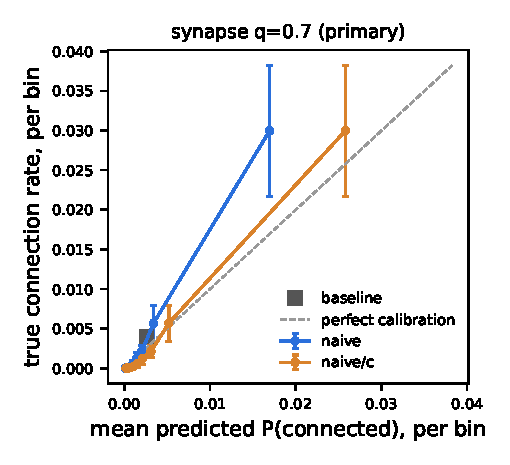
\includegraphics[width=\columnwidth]{../../figures/week9/fig1_reliability_synapse_q0.7_a5.pdf}
\caption{The headline figure as lock note A5 fixes it, without PU: naive and naive/$c$ with the baseline point, synapse dropout $q=0.7$, pooled over 25 runs.}\label{fig:a5}
\end{figure}
\RunDetails
\end{document}
